%% ================================================================
%% # DBIS Databases Hand-in Template
%% 
%% Template for students to hand-in their databases exercise solutions.
%% 
%% [Databases and Information Systems Group](https://dbis.dmi.unibas.ch/)
%%
%% ## Usage
%% 
%% Fill in the required fields and write your submission
%%
%% ## Issues
%%
%% See dbisdbhandin.sty for further information.
%% ================================================================
\documentclass{article}
\usepackage{dbisdbhandin}
\usepackage[english]{babel}
%% ================================================================
%%
%% General Information
%%
%% ================================================================
%%
%% Add your information here
\course       {Databases}
\semester     {Autumn 2025}
\exerciseno   {1}
\studenta     {Ada Lovelace}
\studentb     {Alan Turing}
\studentc     {Edie Windsor} %% Comment if you do the exercises alone



%% ================================================================
%%
%% Common Packages
%%
%% ================================================================
%%
%% Useful common packages for this course

%% Include pdfs into latex
\usepackage{pdfpages}
%% \includepdf[pages=1,pagecommand={\pagestyle{fancy}}]{filename}

%% Drawing everything, with lots of libraries
\usepackage{tikz}
%% A library providing ER prefabs
\usetikzlibrary{er}
\usetikzlibrary{positioning,arrows.meta}
%% ================================================================
%%
%% Custom Packages
%%
%% ================================================================
%%
%% Add custom packages below:
%%

% \usepackage{mypackage}

%% ================================================================
%%
%% Custom Commands
%%
%% ================================================================
%%
%% DRY: Use commands when you use something often or you'd like
%% to define it only once
%%

\newcommand*{\TikZ}{Ti\textit{k}Z}


\begin{document}
%% Required for the title
\printfront
%% ================================================================
%%
%% Description
%%
%% ================================================================

This template showcases various useful latex commands and setups.
Remove this for your actual hand-in.

%% ================================================================
%%
%% Your Solution
%%
%% ================================================================
%%
%% Add your solution below
\task{}
If a tasks asks for an ER diagram, one could use \verb|\usetikzlibrary{er,positioning,arrows.meta}| in the preamble and some code to produce such ER diagrams:
\begin{center}
    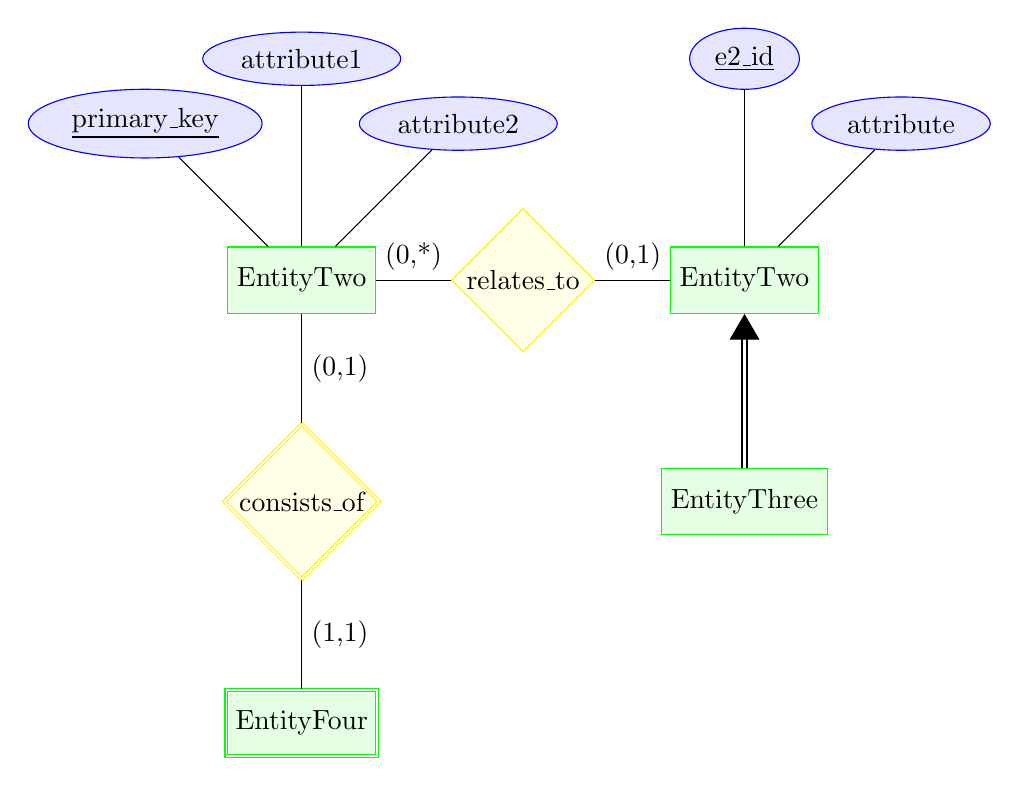
\begin{tikzpicture}[
    every entity/.style={draw=green, fill=green!10, text=black},
    every attribute/.style={draw=blue, fill=blue!10, text=black},
    every relationship/.style={draw=yellow, fill=yellow!10, text=black},
    node distance=8em
    ]
    %% Entity One
    \node[entity](e1){EntityTwo};
    \node[attribute](e1id)[above left of=e1]{\underline{primary\_key}} edge (e1);
    \node[attribute](att1)[above of=e1]{attribute1} edge (e1);
    \node[attribute](att2)[above right of=e1]{attribute2} edge (e1);

    %% Relation, including cardinality
    \node[relationship](rel)[right of=e1]{relates\_to} edge node [auto,swap]{(0,*)}(e1);

    %% Entity Two, including cardinality
    \node[entity](e2)[right of=rel]{EntityTwo} edge node [auto,swap] {(0,1)}(rel);
    \node[attribute](e2id)[above of=e2]{\underline{e2\_id}} edge (e2);
    \node[attribute](e2attr)[above right of=e2]{attribute} edge (e2);

    %% Entity Three, with an IS-A relation to Entity Two (i.e. inheritance)
    \node[entity](e3)[below of=e2]{EntityThree};
    % For Specialization: e3 is a specialization of e2 (i.e. a child of)
    \draw[double distance=.05cm,-Triangle] (e3) -- (e2); % You might want to adjust the double distance value

    %% WEAK Relation, with WEAK Entity
    \node[relationship, double distance=.02cm](rel2)[below of=e1]{consists\_of} edge node[auto,swap]{(0,1)}(e1);
    \node[entity, double distance=.02cm](e4)[below of=rel2]{EntityFour} edge node[auto, swap] {(1,1)}(rel2);
    \end{tikzpicture}
\end{center}

However, it is not \emph{required} to use \TikZ{} for ERs. One can also use external services such as \\
\url{https://www.diagrams.net/} to create PDF documents of ERs.
These can then be inserted into the hand-in using

 \verb|\includepdf[pages=1,pagecommand={\pagestyle{fancy}}]{filename}|

 to include the PDF document \verb|filename|.
It is important to use the pagestyle \emph{fancy}, so that the header is also on the included page. Furthermore, please ensure that your PDF version (or image) of the ER diagram is \textbf{readable}.

\task{}
Relational algebra is a treat with \LaTeX, as can be seen in~\Cref{eq:ans}:

\begin{equation}
\label{eq:ans}
\pi\left[Attribute1,Attribute2\right](\sigma\left[Attribute=Something\right](Entity1) \Join Entity2)
\end{equation}

Other useful symbols related to Relational Algebra are union ($\cup$), intersection ($\cap$), logical and $\land$ and `not equals' ($\not=$).

Also, in regards of Relational Algebra, have a look at:\\
\begin{center}
\begin{tabbing}
    Entity1 \qquad\qquad\= (\uline{PKE1})\\
    Entity2 \> (\uline{PKE2},Attribute)\\
    relation \> (\uline{\uwave{PKE1}, \uwave{PKE2}})
\end{tabbing}    
\end{center}

\task{}
At one point in time, you might want to include SQL snippets to a solution.
One way to do so would be by having an SQL file close by and use \verb|\lstinputlisting| -- provided by the \verb|listings| package.

\lstinputlisting[language=SQL,frame=single,numbers=left,numberstyle=\tiny]{example.sql}

\task{}

It is also possible to 
%% Note that this example (SQL + operator trees) is borrowed from the lecture slides.
\begin{enumerate}[a)]
    \item have SQL in \LaTeX:
    \begin{lstlisting}[language=SQL,frame=single,numbers=left,numberstyle=\tiny]
SELECT DISTINCT DESCR
FROM Products P, Orders O
WHERE O.PId = .PId
AND CIty = :c AND Weight > :w
AND Amount > :a
    \end{lstlisting}
    
    \item Operator Trees using \TikZ:\\
    \setlength{\columnseprule}{1pt}
    \begin{multicols}{2}
        \begin{center}
            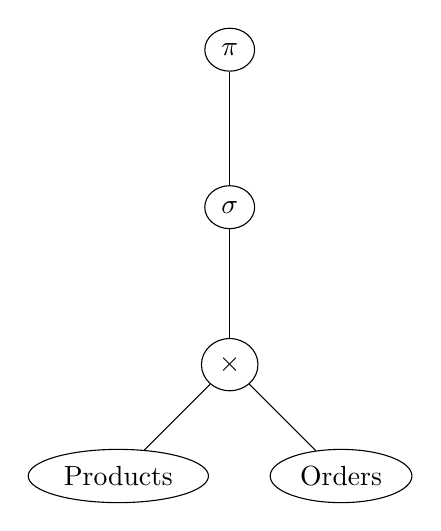
\begin{tikzpicture}[
            node distance = 2cm,
            op/.style={ellipse,draw}]
            \node[op](pi){$\pi$};
            \node[op,below of=pi](sigma){$\sigma$};
            \node[op,below of=sigma](cross){$\times$};
            \node[op,below left of=cross](products){Products};
            \node[op,below right of=cross](orders){Orders};
            
            \path (pi)    edge (sigma)
            (sigma) edge (cross)
            (cross) edge (products)
            (cross) edge (orders);
            \end{tikzpicture}
        \end{center}
        \columnbreak
        
        \begin{center}
            \begin{tikzpicture}[
            node distance = 2cm,
            op/.style={ellipse,draw}]
            \node[op](pi){$\pi$};
            \node[op,below of=pi](join){$\Join$};
            \node[op,below left of=join](left){$\sigma$};
            \node[op,below right of=join](right){$\sigma$};
            \node[op,below of=left](products){Products};
            \node[op,below of=right](orders){Orders};
            
            \path (pi)    edge (join)
            (join)  edge (left)
            (join)  edge (right)
            (left)  edge (products)
            (right) edge (orders);
            \end{tikzpicture}
        \end{center}        
    \end{multicols}
\end{enumerate}

\task{}
If you need more information regarding \LaTeX, visit one of the following places:

\begin{itemize}
    \item \url{https://en.wikibooks.org/wiki/LaTeX}
    \item \url{https://www.overleaf.com/learn}
\end{itemize}

We recommend using Overleaf to collaboratively edit \LaTeX{} documents.
\end{document}
